\documentclass{standalone}
\begin{document}
	\begin{frame}[noframenumbering]{Max Eigenvalues Map}{Bronchial Structure Removal}
		\begin{columns}[b]
		
			\begin{column}{.4\textwidth}
				\centering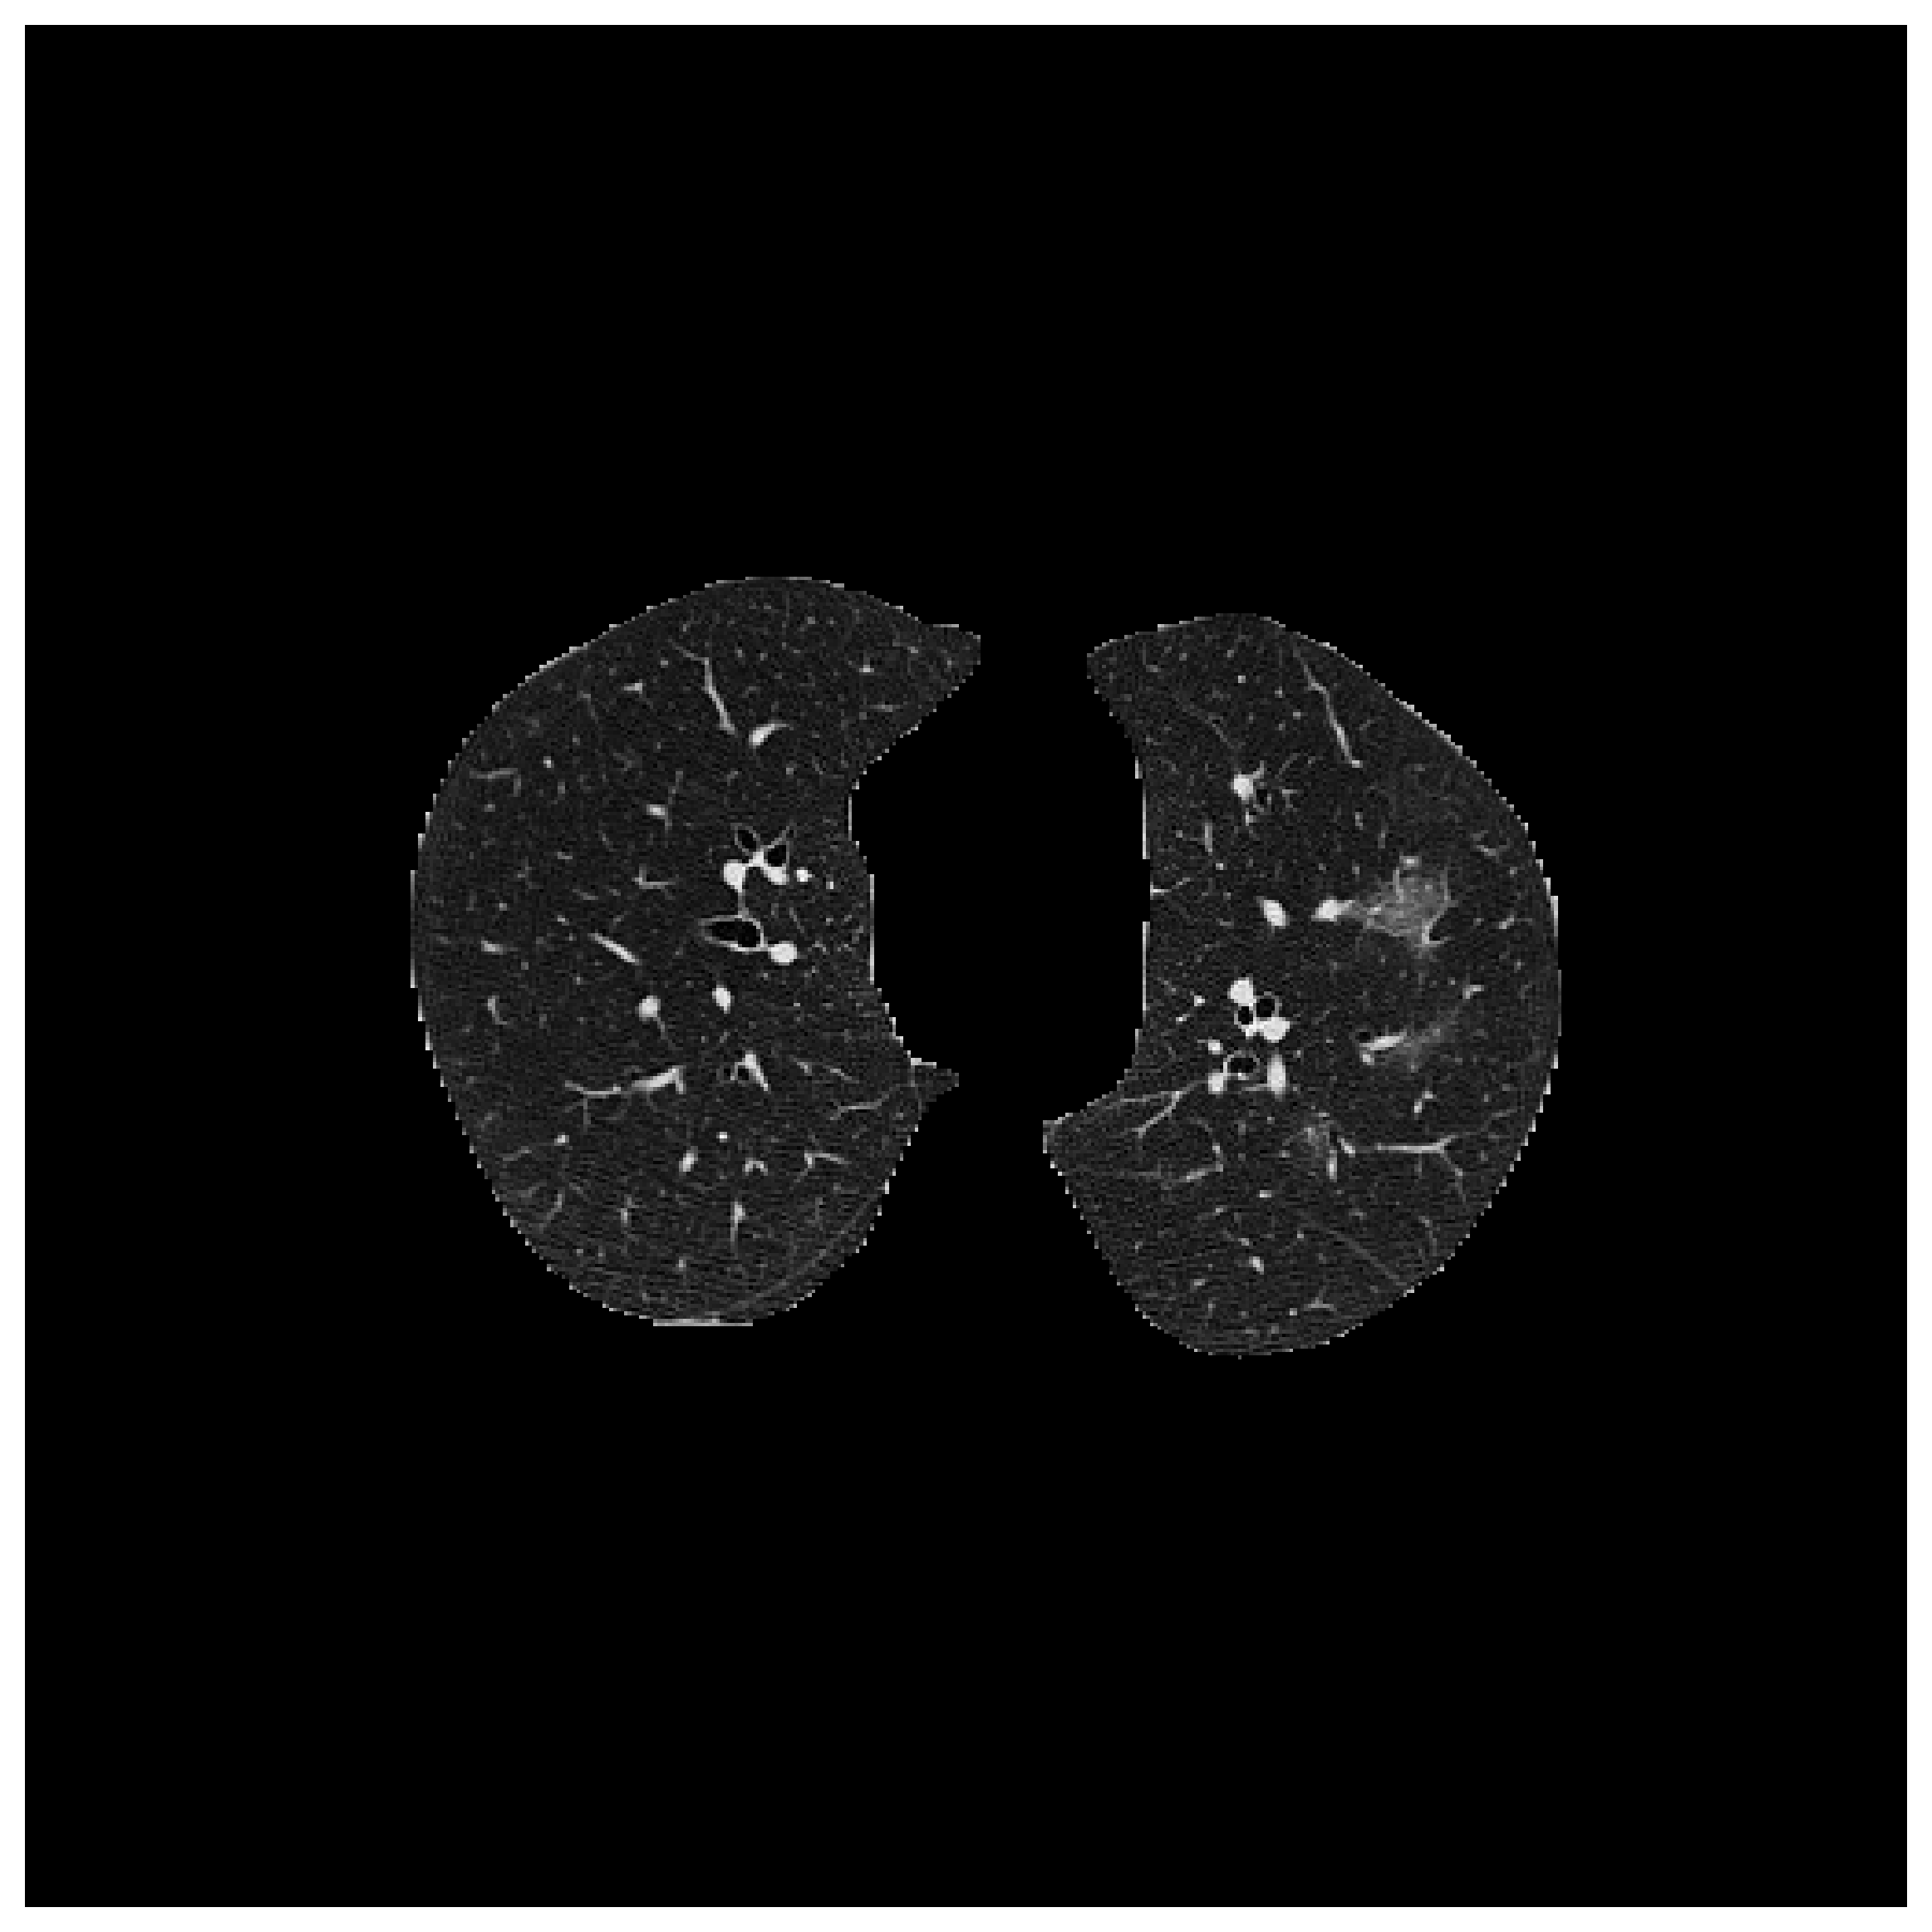
\includegraphics[width=.7\linewidth]{./img/Lung_2}
				\centering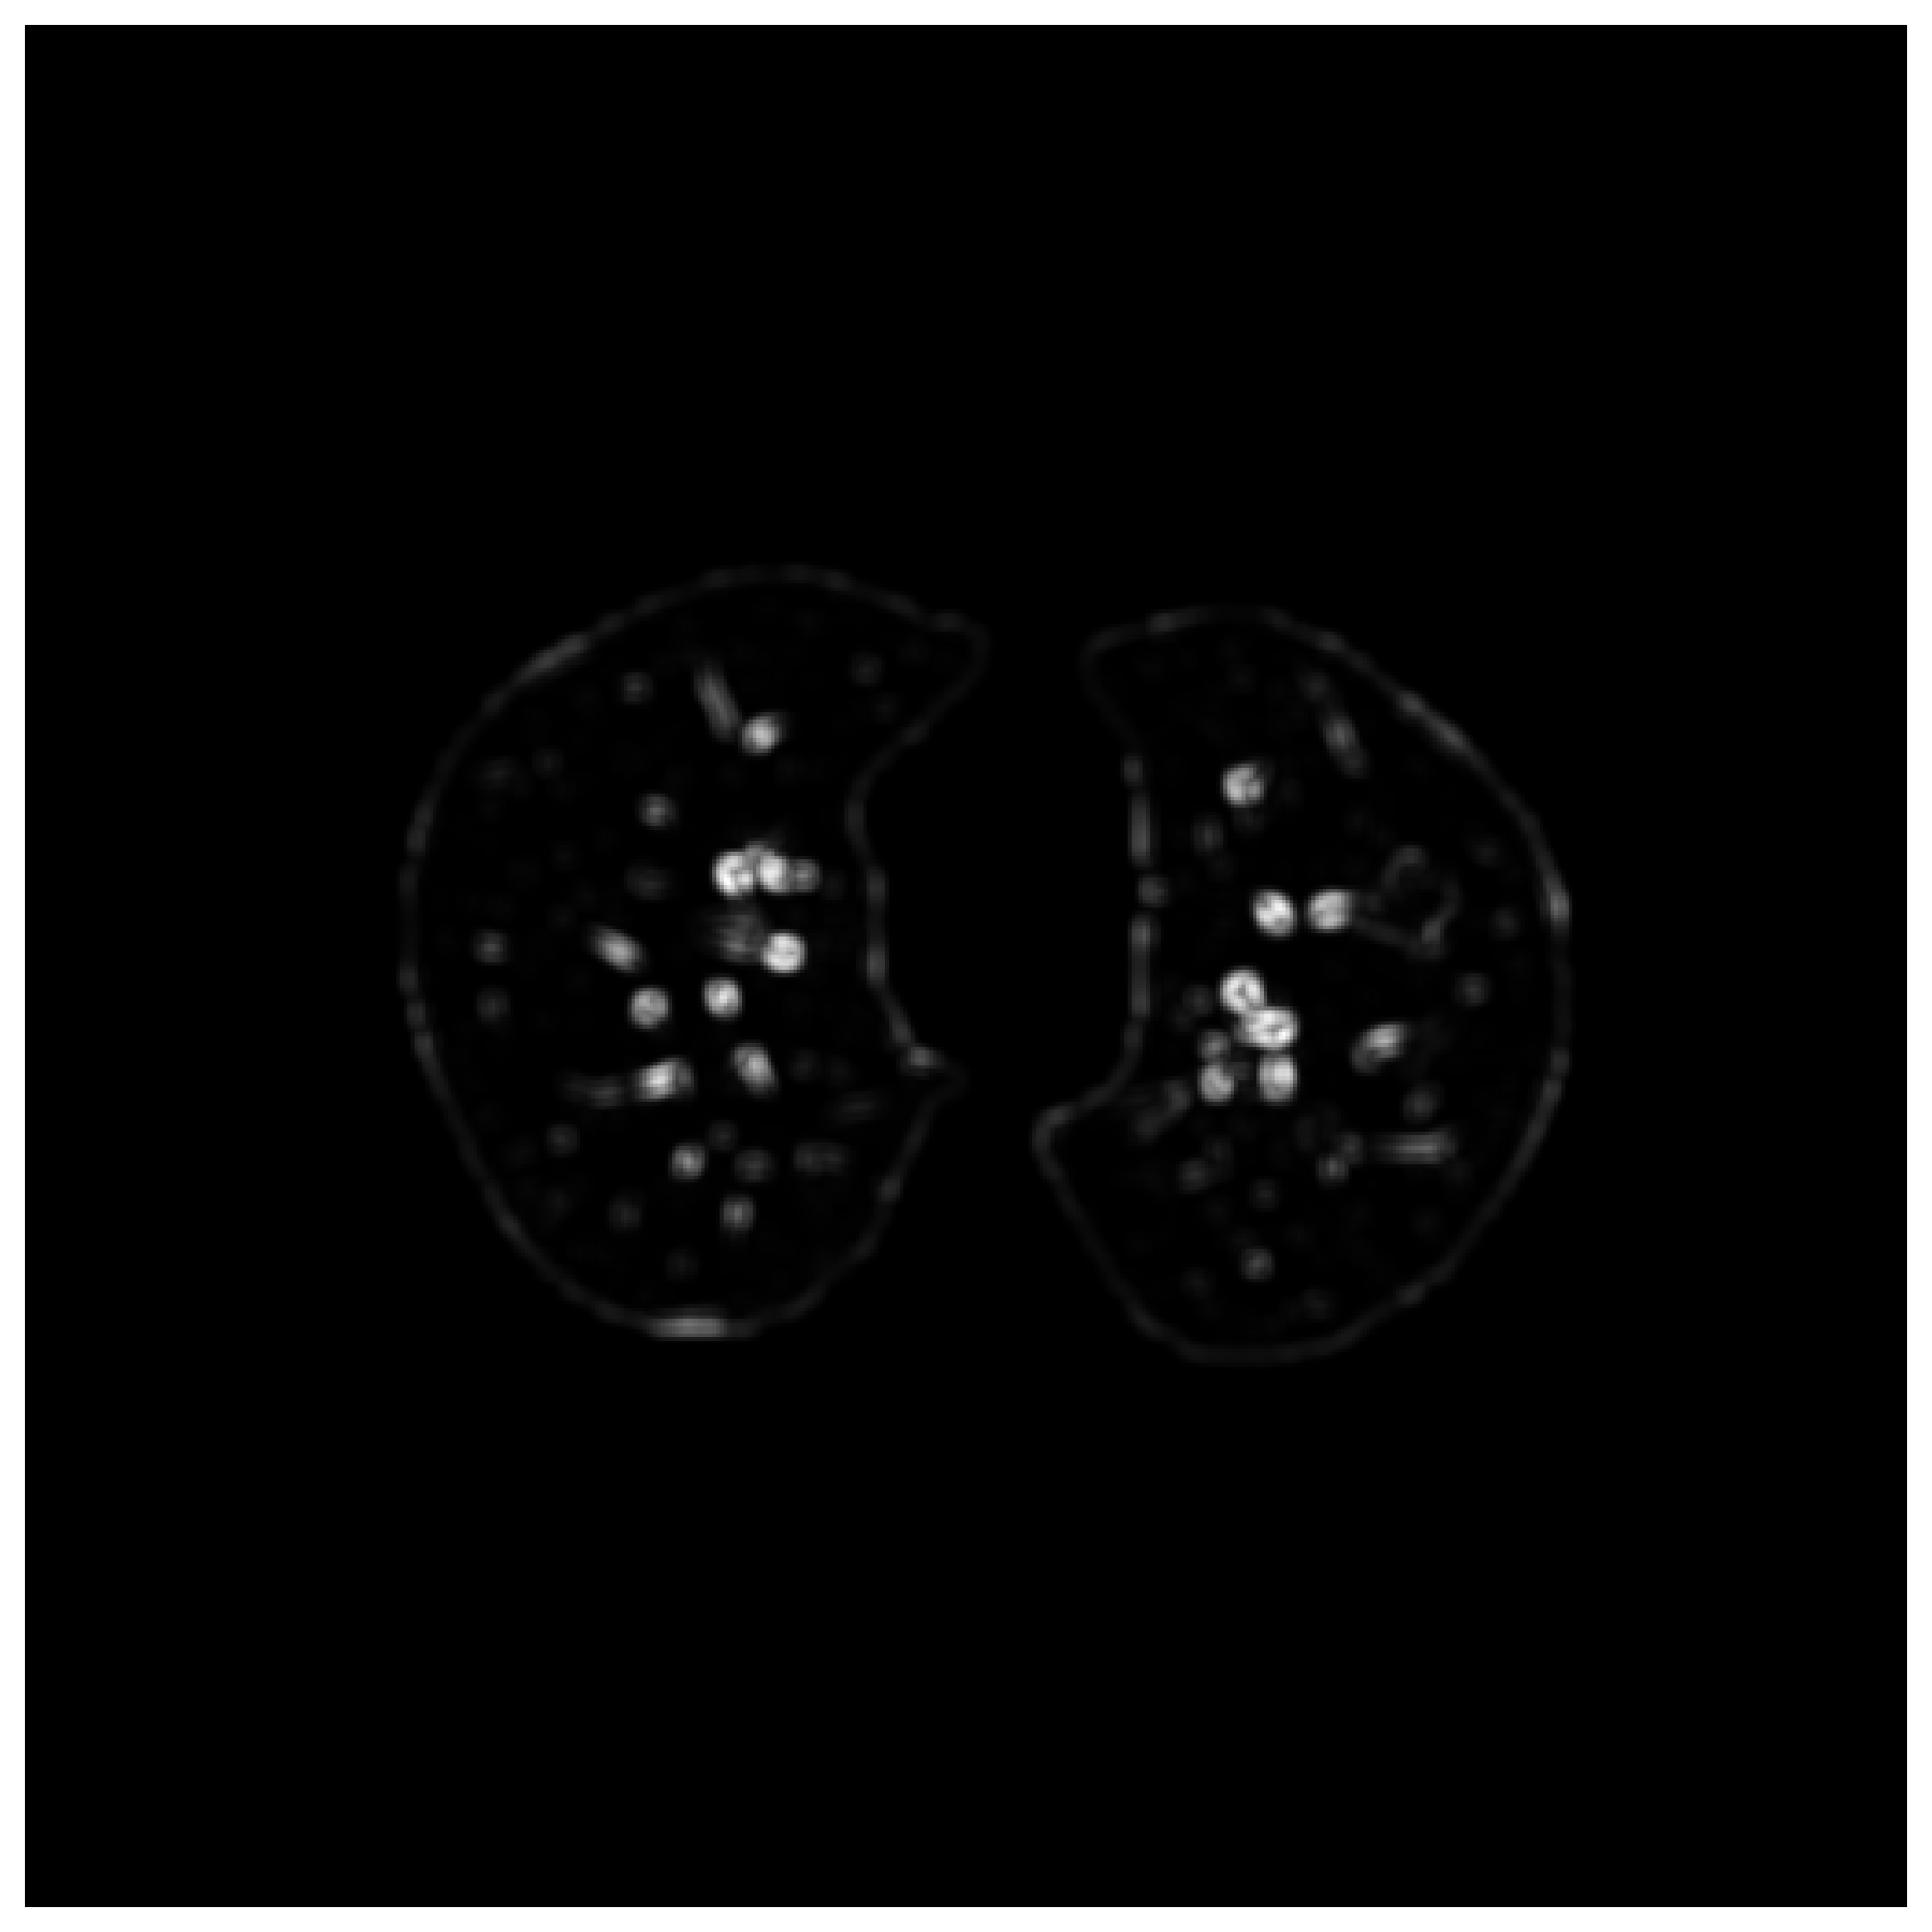
\includegraphics[width=.7\linewidth]{./img/eigmap}
			\end{column}
			\begin{column}{.4\textwidth}
			%\begin{scriptsize}	

				\begin{equation*}
					M = \begin{bmatrix} \sum _{S(p)}(\frac{dI}{dx})^2 & \sum _{S(p)}\frac{dI}{dx}\frac{dI}{dy} \\ \sum _{S(p)}\frac{dI}{dx}\frac{dI}{dx}& \sum _{S(p)}(\frac{dI}{dy})^2 \end{bmatrix}
				\end{equation*}
			%\end{scriptsize}	
		
			\centering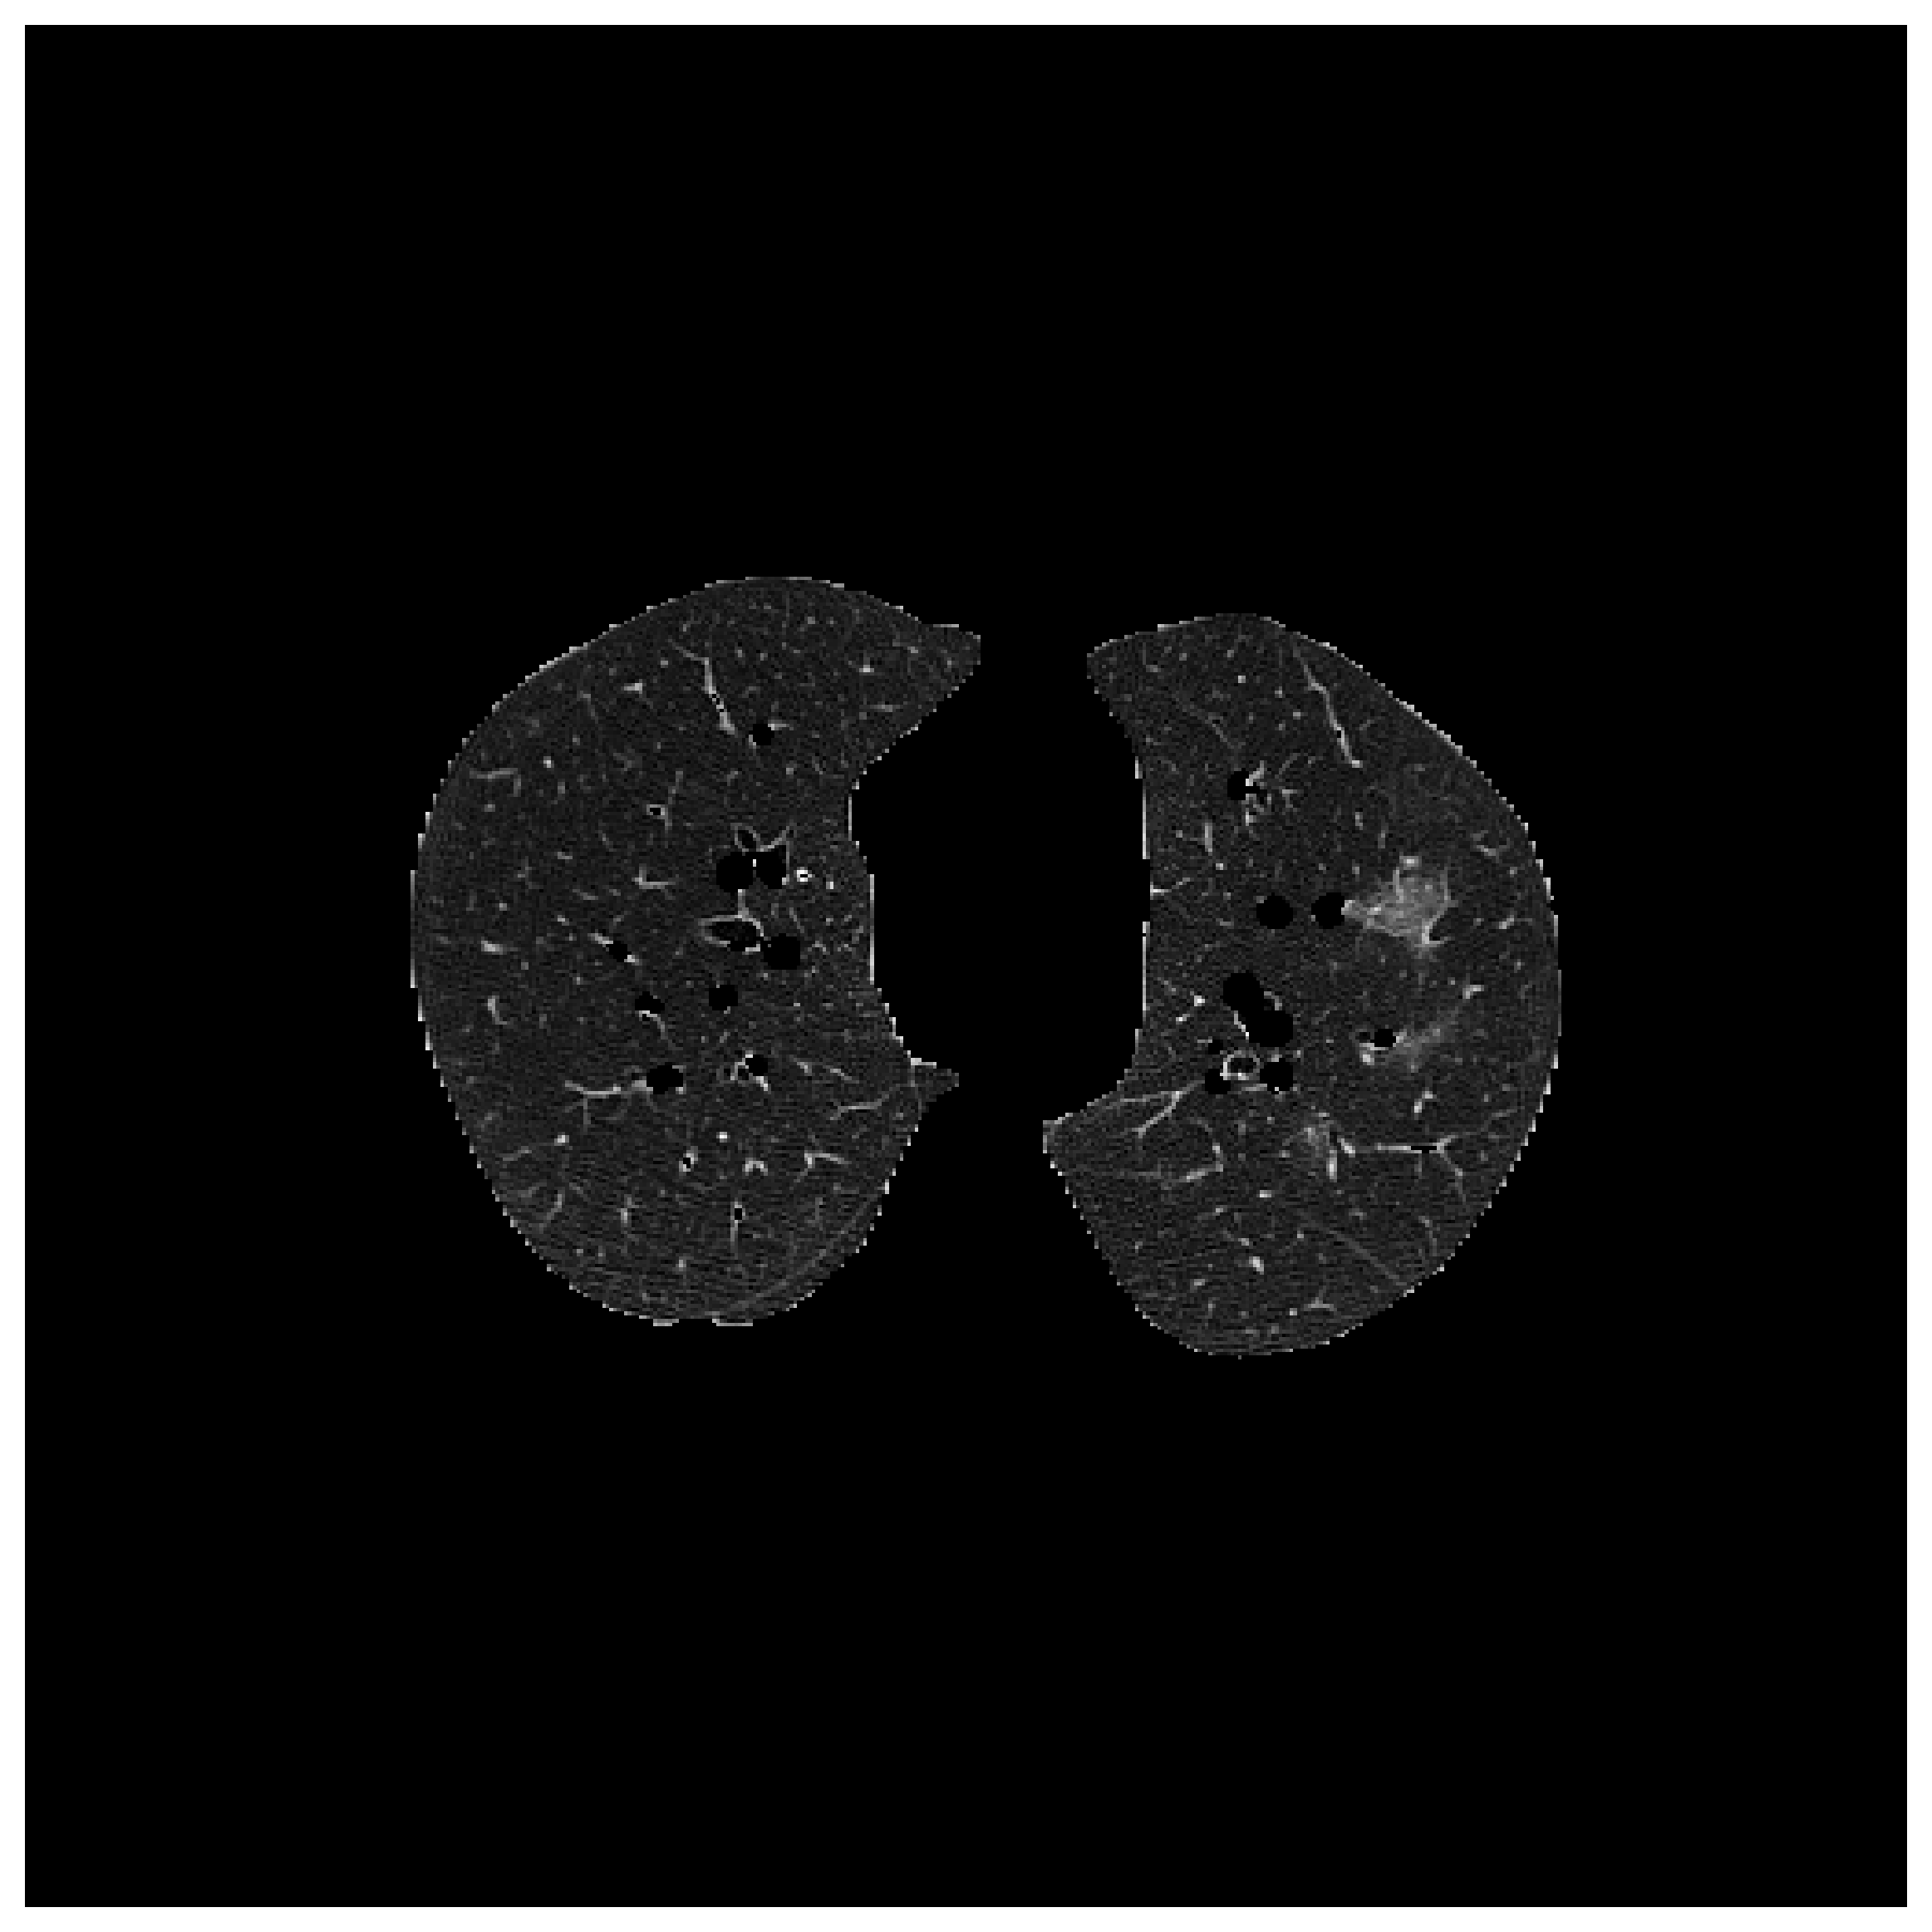
\includegraphics[width=.7\linewidth]{./img/NoBr}
		\end{column}
		\end{columns}
	\end{frame}
\end{document}